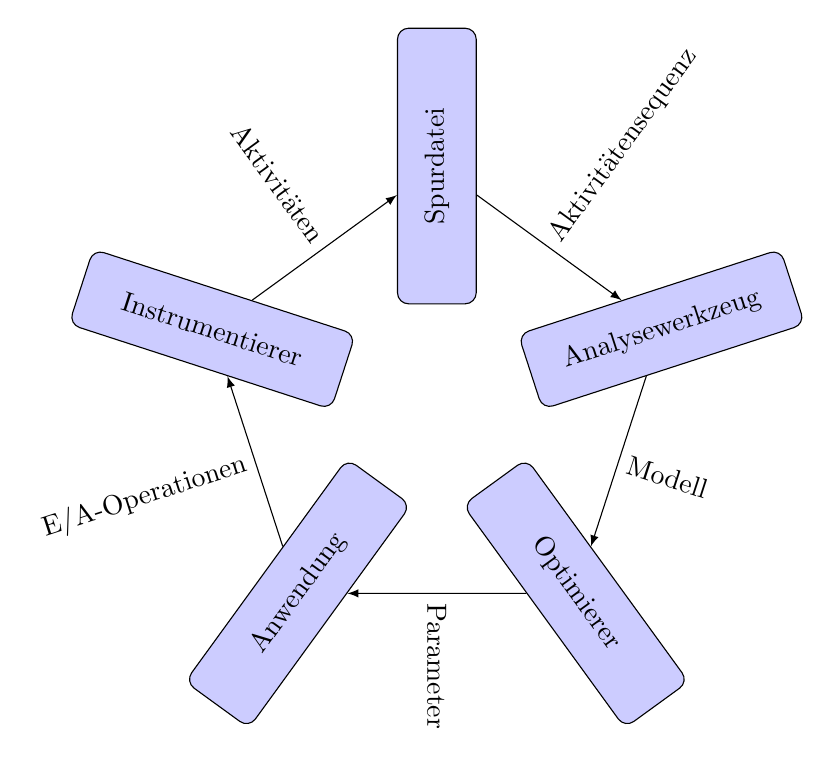
\begin{tikzpicture}
	[
		remember picture,
		>=latex reversed,
		phase/.style={draw,rounded corners, fill=blue!20, align=center, minimum height=1cm, minimum width=3.5cm},
		node distance=5mm and 5mm
	]

	\def\dist{3cm}

	\coordinate
	[]
		(center) at (0,0);

		\path (0,0) (90:\dist) node
		[phase, rotate=90, label={[align=center]270:{}}]
		(phase00)
		{Spurdatei};

		\path (0,0) (18:\dist) node
		[phase, rotate=18, label={[align=center]270:{}}]
		(phase01)
		{Analysewerkzeug};

		\path (0,0) (-54:\dist) node
		[phase, rotate=-54, label={[align=center]270:{}}]
		(phase02)
		{Optimierer};

		\path (0,0) (234:\dist) node
		[phase, rotate=54, label={[align=center]270:{}}]
		(phase03)
		{Anwendung};

		\path (0,0) (162:\dist) node
		[phase, rotate=-18, label={[align=center]90:{}}]
		(phase04)
		{Instrumentierer};

		\path
		[->, >=latex]
		(phase00)       edge node[rotate=54, right] (sequenz) {Aktivitätensequenz}    (phase01)
		(phase01)       edge node[rotate=-18, right] (model) {Modell}   (phase02)
		(phase02)       edge node[rotate=-90, right] (params) {Parameter}    (phase03)
		(phase03)       edge node[rotate=18, left] (ops) {E/A-Operationen}(phase04)
		(phase04)       edge node[rotate=-54, left] (act) {Aktivitäten}   (phase00);


\end{tikzpicture}
